\documentclass{article}

\usepackage[utf8]{inputenc}
\usepackage[colorlinks,linkcolor=red]{hyperref}
\usepackage{graphicx}

\title{
    {Paper Note}\\
    {\large "Model-Agnostic Boundary-Adversarial Sampling for Test-Time Generalization in Few-Shot learning"}
}
\author{Lisen Dai}
\date{Oct 2020}

\begin{document}

\maketitle

\section{General Discription of Few-shot}
Paper link:\href{https://www.ecva.net/papers/eccv_2020/papers_ECCV/papers/123460579.pdf}{ECCV}
\subsection{Few-shot problem}
Few-shot learning is a general name for tasks in which people hope
to train a machine learning model with just very small amount of data. \newline

\subsection{Previous Research}
1. \textbf{Data augmentation}. Generating fake labaled data. \newline
2. Distance metric methods. \newline
3. Meta-learning methods. \newline

\subsection{Limitations of data augmentation few-shot}
1. Such methods learn to generate additional examples with the 
meta-training set, and thus may not be effective if meta-test domains are far from the meta-training domain. \\
2. Since they do not update the trained parameters of the base 
classifier models at test time, they have no chance to correct the 
errors that exist in the base classifiers (e.g. overfitting of the embedding functions to the meta-training set). \\
3. These methods need to be re-trained for each base classifier 
to generate fake labeled data optimal for the base model. \\

\section{Innovative Designs}
A novel model-agnostic sample generation approach named \textbf{MABAS} (Model-Agnostic Boundary-Adversarial Sampling). \\
\subsection{Test-time Fine-tuning of Embedding Functions}
Since each meta-test task consists of the classes that are never seen during metatraining, 
it is a common approach in few-shot learning to fine-tuning the learned parameters using the
support samples of the novel task. This work aims at fine-tuning the learned parameters of the
base few-shot learner adaptively to novel tasks but limited to update the parameters of the
embedding function (or the feature extractor). 
\subsection{Fine-tuning by Boundary-Adversatial Samples}
Once we have the adversatial samples, we can update the parameter $\phi$ of embedding function via \underline{gradient descent}. The fine-tuning loss $\mathcal{L}^{fine-tune}$ is defined as: \\
$$
\mathcal{L}^{fine-tune}(\mathcal{S}, \phi) := \mathcal{L}^{adv}(\mathcal{S}, \phi) + \eta \cdot \frac{1}{\mathcal{S}}\sum_{(\textbf{x},y)}\in\mathcal{S}{\Vert}f_{\phi}(\textbf{x}){Vert}^2,
$$
and, 
$$
\mathcal{L}^{adv}(\mathcal{S}, \phi) = 
\frac{1}{\mathcal{S}} 
\sum_((\textbf{x}, y) \in \mathcal{S})[
    \frac{1}{K - 1} \sum_{k\prime \neq y} 
        \{\alpha_{\textbf{x},y} - 
        \min{
            m(\textbf{z}_{y, k\prime}^{adv}, y, k | \psi, \mathcal{S})
            } 
        \}_+
    ]
$$
where,
$
\alpha_{\textbf{x}, y} =
\frac{1}{K - 1} 
\sum_{k \neq y} 
m 
(\textbf{z}, y, k 
|
\phi,
\mathcal{S}
)
$
\\
feature: not only prevents the exces- sive expansion 
of the supports’ embedding space but also stabilizes 
the updates of the embedding space.\\
Below is an illustration picture of the MABAS method.\\
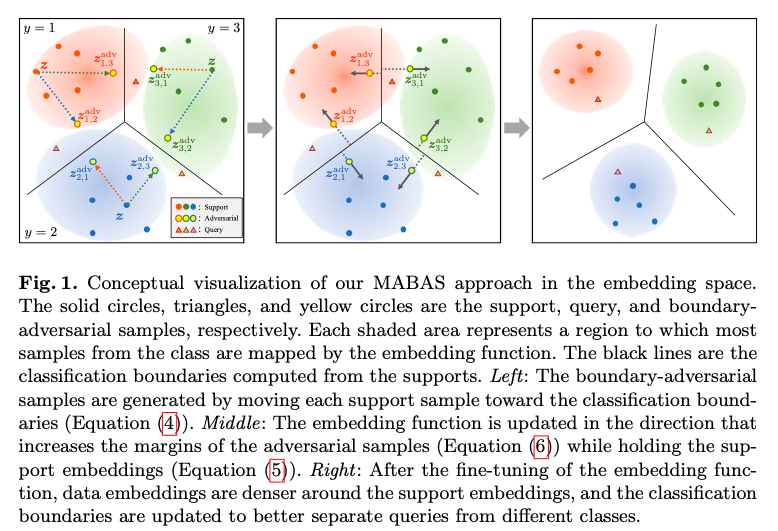
\includegraphics[scale=0.6]{src/img/MABAS Illustration.jpg}\\

\section{Other Applications of Few-shot}
To show the flexibility and generality of our MABAS approach, 
this paper applies it to three representative few-shot learning methods: \\
1. MetaOptNet \\
2. Few-Shot without Forgetting \\
3. Standard Transfer Learning \\

In each method, the paper give out the original equation of implementation 
and then the three ways below about how to optimize it by MABAS: \\
1. Boundary-adversarial fine-tuning. \\
2. Variation. \\
3. Setting of $\delta$ \\
And here's an example of \textit{MetaOptNet}: \\
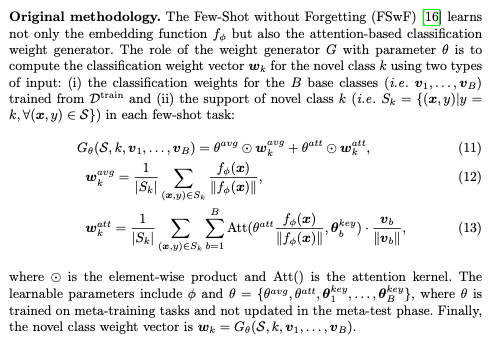
\includegraphics[scale=0.6]{src/img/MetaOptNet1.jpg} \\
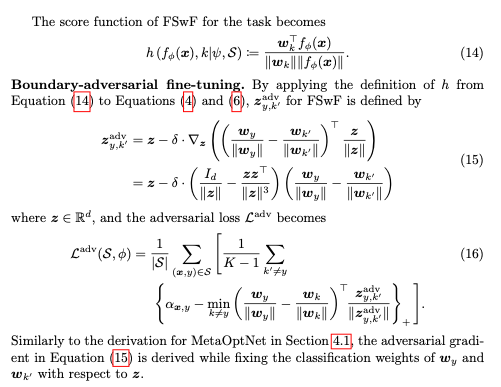
\includegraphics[scale=0.6]{src/img/MetaOptNet2.jpg} \\

\section{Experiment}
\section{setup}
dataset: \\
1. miniImageNet: consists of 100 classes each of which has 600 images with a size of 84 × 84 × 3. It adopts the same class split used by [36, 22]: 64, 16 and 20 classes for training, validation and the test, respectively. \\
2. CIFAR-FS: splits all of the classes in CIFAR100 [20] into 64 training, 16 validation and 20 test sets, respectively. \\
3. FC100: is another CIFAR100-based dataset. Classes are split into 60, 20 and 20 for training, validation and test, respectively. This class split is designed to minimize the overlap of information between all three subsets, to be more challenging than CIFAR-FS for few-shot learning. \\
 
\end{document}